\documentclass[conference]{IEEEtran}

% ── Packages ──────────────────────────────────────────────────────────────────
\usepackage{cite}
\usepackage{amsmath,amssymb,amsfonts}
\usepackage{algorithmic}
\usepackage{algorithm}
\usepackage{graphicx}
\usepackage{textcomp}
\usepackage{xcolor}
\usepackage{booktabs}
\usepackage{multirow}
\usepackage{array}
\usepackage{adjustbox}
\usepackage{tikz}
\usetikzlibrary{positioning,arrows.meta,fit,calc,shapes.geometric}
\usepackage{flushend}
\usepackage[hidelinks]{hyperref}
\usepackage{enumitem}

% IEEE-compatible float placement
\def\BibTeX{{\rm B\kern-.05em{\sc i\kern-.025em b}\kern-.08em T\kern-.1667em\lower.7ex\hbox{E}\kern-.125emX}}

\begin{document}

% ══════════════════════════════════════════════════════════════════════════════
%  TITLE
% ══════════════════════════════════════════════════════════════════════════════

\title{Dual-Branch Spatial-Frequency Fusion for AI-Generated Image Detection: A Cross-Dataset Evaluation with FFT and DCT Spectral Representations}

\author{
\IEEEauthorblockN{Shreyanshu Raj}
\IEEEauthorblockA{Dept.\ of Computer Science \& Eng.\\(Cyber Security)\\
Ramaiah Institute of Technology\\Bengaluru, Karnataka, India\\
1ms24cy073@msrit.edu}
\and
\IEEEauthorblockN{Raj Aryan}
\IEEEauthorblockA{Dept.\ of Computer Science \& Eng.\\(Cyber Security)\\
Ramaiah Institute of Technology\\Bengaluru, Karnataka, India\\
1ms24cy051@msrit.edu}
\and
\IEEEauthorblockN{Meghanshu Kumar}
\IEEEauthorblockA{Dept.\ of Computer Science \& Eng.\\(Cyber Security)\\
Ramaiah Institute of Technology\\Bengaluru, Karnataka, India\\
1ms24cy035@msrit.edu}
}

\maketitle

% ══════════════════════════════════════════════════════════════════════════════
%  ABSTRACT
% ══════════════════════════════════════════════════════════════════════════════

\begin{abstract}
Generative models such as GANs and latent diffusion networks now synthesize images that are perceptually indistinguishable from authentic photographs, posing serious threats to digital trust and media integrity. Existing detectors that rely exclusively on spatial pixel features tend to overfit to the generative pipeline seen during training, while frequency-only methods suffer from limited discriminative power. We present a dual-branch architecture that fuses a pre-trained ResNet-18 spatial backbone with a lightweight spectral CNN operating on log-magnitude 2D-FFT or separable 2D-DCT representations, computed entirely on the GPU without resizing or interpolation artifacts. The pipeline enforces lossless center-cropping, SHA-256 deduplication, and validation-calibrated Youden's $J$ thresholding to ensure leak-free evaluation. Trained on 40{,}000 balanced images from the GRAVEX-200K corpus and evaluated across four heterogeneous datasets, the fused DCT variant attains 0.9268 ROC-AUC on the in-domain test set and achieves 0.9656 ROC-AUC with 90.97\% accuracy in zero-shot cross-dataset transfer to 140K Real and Fake Faces, outperforming both single-branch baselines. Systematic ablation over three random seeds, two spectral transforms, and two evaluation protocols quantifies the contribution of each component and identifies spectral resolution mismatch as a primary failure mode in cross-domain settings.
\end{abstract}

\begin{IEEEkeywords}
AI-generated image detection, spatial-frequency fusion, discrete cosine transform, fast Fourier transform, cross-dataset generalization, deepfake forensics
\end{IEEEkeywords}

% ══════════════════════════════════════════════════════════════════════════════
%  I. INTRODUCTION
% ══════════════════════════════════════════════════════════════════════════════

\section{Introduction}
\label{sec:intro}

The rapid maturation of generative adversarial networks (GANs)~\cite{goodfellow2014gan} and latent diffusion models (LDMs)~\cite{rombach2022ldm} has democratized photorealistic image synthesis. A single text prompt can now produce high-resolution photographs that defeat both casual human inspection and legacy forensic tools. The societal consequences---misinformation campaigns, identity fraud, non-consensual face synthesis, and manipulation of medical or legal evidence---demand reliable, automated detection mechanisms that generalize across generative architectures and image domains.

Spatial-domain detectors built on convolutional neural networks (CNNs) extract texture, edge, and semantic features that often correlate with the specific upsampling or denoising artifacts of a single generator. As Chandrasegaran~\emph{et~al.}~\cite{chandrasegaran2021fourier} demonstrated, these spectral peaks can be eliminated by simply replacing the transposed-convolution upsampler with bilinear interpolation, collapsing frequency-based detectors trained on those cues. Corvi~\emph{et~al.}~\cite{corvi2023intriguing} subsequently showed that classifiers trained on GAN outputs perform near chance when confronted with diffusion-synthesized imagery, confirming that generator-specific overfitting remains the central failure mode.

Frequency-domain approaches attempt to bypass semantic content and capture low-level synthesis fingerprints. Bammey~\cite{bammey2023synthbuster} extracted Fourier peak features from cross-difference residuals, while Das~\emph{et~al.}~\cite{das2023dctfade} analysed high-frequency DCT coefficients across video frames. Both methods are lightweight and interpretable, yet their accuracy degrades on unseen generators and under JPEG compression. More recent dual-stream architectures---SFFNet~\cite{wang2025sffnet}, SFCL~\cite{qiao2025sfcl}, CSFD~\cite{li2025csfd}, and SFANet~\cite{guo2025sfanet}---fuse spatial and spectral branches with cross-attention or channel-attention mechanisms. Despite strong in-domain results, these methods typically resize inputs to a fixed resolution, an operation that introduces resampling artifacts into the frequency spectrum and confounds the very signal the detector seeks.

This paper addresses three open gaps: (1)~the lack of controlled ablation isolating the contribution of each domain under identical preprocessing, (2)~the absence of interpolation-free evaluation protocols that preserve native spectral statistics, and (3)~insufficient cross-dataset generalization benchmarks spanning diverse generative paradigms (diffusion, GAN, autoencoder) at heterogeneous resolutions. The principal contributions are:

\begin{itemize}[leftmargin=*,nosep]
\item A dual-branch architecture coupling a pre-trained ResNet-18 spatial encoder with a lightweight 4-stage CNN operating on log-magnitude 2D-FFT or orthonormal separable 2D-DCT spectra, with optional Hann windowing, variable-resolution support via global average pooling, and projection-based capacity balancing before late fusion.

\item A leak-free evaluation pipeline that employs SHA-256 byte-level deduplication, lossless center-cropping without interpolation, and validation-only Youden's~$J$ threshold calibration, enforced across four public Kaggle datasets totalling 255{,}264 verified images.

\item A systematic cross-dataset transfer evaluation under two controlled resolution protocols---Protocol~C (common $32{\times}32$ crop) and Protocol~N (native per-dataset crop)---demonstrating that the fused model achieves 0.9656 ROC-AUC on zero-shot face synthesis detection while identifying spectral resolution mismatch as the dominant failure mode on low-resolution target domains.

\item A reproducible, seed-controlled experimental framework reporting mean $\pm$ standard deviation over three seeds for all primary metrics, with open-source code and pre-trained checkpoints.
\end{itemize}

The remainder of this paper is organized as follows. Section~\ref{sec:related} surveys relevant spatial, frequency, and hybrid detection methods. Section~\ref{sec:method} details the proposed architecture and preprocessing pipeline. Section~\ref{sec:setup} describes the experimental configuration, datasets, and evaluation metrics. Section~\ref{sec:results} presents and analyses the results. Section~\ref{sec:conclusion} concludes with future directions.


% ══════════════════════════════════════════════════════════════════════════════
%  II. RELATED WORK
% ══════════════════════════════════════════════════════════════════════════════

\section{Related Work}
\label{sec:related}

We organize prior work into three thematic categories: frequency-domain forensics, spatial-frequency fusion architectures, and physics-based or self-supervised detection paradigms.

\subsection{Frequency-Domain Forensics}

Early spectral forensics exploited the observation that CNN-based generators produce systematic high-frequency anomalies due to upsampling operations. Chandrasegaran~\emph{et~al.}~\cite{chandrasegaran2021fourier} traced these Fourier spectrum discrepancies to the zero-insertion step in transposed convolutions and showed that replacing them with interpolation-based upsampling eliminates the spectral peaks entirely, reducing detector accuracy from above 99\% to near chance. This foundational result established that spectral cues are architecture-dependent rather than inherent to generative modelling.

Bammey~\cite{bammey2023synthbuster} developed Synthbuster, which applies cross-difference filtering followed by FFT peak extraction and gradient-boosted classification. Despite reaching an MCC of 0.872 on known generators, generalization to unseen diffusion models such as DALL-E~2 dropped to an MCC of 0.478, and performance degraded below JPEG quality~70. Das~\emph{et~al.}~\cite{das2023dctfade} proposed DCT-FADE for video forensics, detecting elevated variance in high-frequency DCT coefficients across consecutive frames; however, their approach requires pristine reference footage and cannot operate in a fully blind setting.

Li~\emph{et~al.}~\cite{li2024masksim} introduced MaskSim, a semi-white-box method that detects synthetic images through masked Fourier spectrum similarity analysis using a fine-tuned DnCNN denoiser. While the approach achieved 88.3\% average AUC across diffusion models, its fixed spectral masks fail when synthetic images undergo rescaling. Bilbis~\emph{et~al.}~\cite{bilbis2025dctvsfft} systematically compared DCT and FFT features paired with parallel ResNet-18 streams across twelve JPEG quality levels, finding that DCT features exhibit 24.7\% less accuracy degradation than FFT under heavy compression---a result that informs our inclusion of both transforms.

\subsection{Spatial-Frequency Fusion Architectures}

Recent work has converged on dual-stream architectures that jointly exploit spatial and spectral representations. Wang~\cite{wang2025sffnet} proposed SFFNet, coupling an EfficientNet-B3 spatial branch with high-frequency residual blocks and frequency channel learning, achieving 94.6\% mean accuracy on DiffusionForensics. Qiao~\emph{et~al.}~\cite{qiao2025sfcl} developed SFCL, a framework that extracts local frequency features using block-wise DCT with multi-scale convolutions alongside a global frequency branch, then fuses them with spatial features through cross-modal attention. Li~\emph{et~al.}~\cite{li2025csfd} partitioned images into strong- and weak-texture regions before spectral processing, using weighted channel attention to aggregate frequency components. Guo~\emph{et~al.}~\cite{guo2025sfanet} combined wavelet-based feature decoupling with dual-attention and cross-modality fusion in SFANet.

Yang~\emph{et~al.}~\cite{yang2025multicue} extended the fusion paradigm by adding chromatic phase features extracted from YCbCr channels alongside spatial and frequency branches, reaching 80.0\% average cross-dataset AUC. Liu~\emph{et~al.}~\cite{liu2024atsc} proposed ATSC, which employs input-adaptive dynamic convolutions for texture mining and adaptive DCT coefficient selection, attaining 82.35\% video-level AUC on Celeb-DF-v2 when trained only on FaceForensics++. Pradeepan and Raj~\cite{pradeepan2024medical} demonstrated the clinical relevance of spatial-frequency fusion by applying dual-stream EfficientNet-B0 and Haar DWT processing to detect synthetic nodule insertion in lung CT scans, achieving 99.6\% accuracy.

A common limitation across these methods is the reliance on fixed-resolution input resizing (typically $256{\times}256$), which introduces resampling artifacts into the frequency domain. Our work eliminates this confound through interpolation-free center-cropping.

\subsection{Alternative Detection Paradigms}

Several approaches depart from direct pixel or frequency classification. Wu and Li~\cite{wu2024prnu} leveraged Photo Response Non-Uniformity (PRNU), a physical sensor noise pattern absent in synthetic imagery, achieving 82.2\% average accuracy across eleven generators. Wang~\emph{et~al.}~\cite{wang2023fingerprint} addressed cross-generator generalization by augmenting in the forensic fingerprint domain rather than pixel space, disentangling spatial content from residual high-frequency fingerprints via an autoencoder and achieving 84.7\% mean cross-GAN accuracy. Tan~\emph{et~al.}~\cite{tan2023lgrad} proposed LGrad, which classifies input gradients of a fixed pre-trained CNN rather than raw pixels, achieving 86.3\% cross-generator accuracy but suffering under JPEG compression. Hooda~\emph{et~al.}~\cite{hooda2024d4} addressed adversarial robustness by partitioning DCT coefficients into disjoint frequency bands with independent classifiers, reducing black-box attack success from above 90\% to 28\%.

Karageorgiou~\emph{et~al.}~\cite{karageorgiou2025spai} framed detection as anomaly identification against the spectral distribution of authentic images, using self-supervised masked spectral pre-training on a ViT-B/16 backbone to reach 91.0\% average AUC across thirteen generators. Wang~\emph{et~al.}~\cite{wang2025mifae} reformulated face forgery detection as anomaly modelling through masked image-frequency autoencoders. Balakrishnan~\emph{et~al.}~\cite{balakrishnan2025spectraclip} combined frozen CLIP ViT-B/32 embeddings with radial FFT power spectrum metrics, reaching 94.94\% accuracy with XGBoost classification. Zhong~\emph{et~al.}~\cite{zhong2026selfsup} proposed self-supervised detection using camera EXIF metadata and high-frequency residuals, demonstrating strong generalization without generator-specific supervision. Uddin~\emph{et~al.}~\cite{uddin2025lowres} combined multi-scale DCT with Vision Transformer self-attention for low-resolution deepfake detection, and Sabareshwar~\emph{et~al.}~\cite{sabareshwar2024lightweight} designed a 185K-parameter depthwise-separable CNN operating on global DCT coefficients for edge deployment.

Ahire~\emph{et~al.}~\cite{ahire2025sffnet} and Deng~\emph{et~al.}~\cite{deng2023wavelet} further confirmed the complementarity of spatial and frequency information, the former through spatial-frequency fusion and the latter through learnable wavelet lifting blocks that capture diffusion-specific sub-band anomalies invisible in Fourier analysis.

\subsection{Research Gap}

Despite substantial progress, three gaps persist. First, most dual-stream methods resize inputs before spectral analysis, corrupting the frequency statistics they aim to exploit. Second, controlled ablations isolating the marginal contribution of each branch under identical, interpolation-free preprocessing are rare. Third, cross-dataset evaluations seldom account for resolution heterogeneity between source and target domains, conflating spectral mismatch with genuine generalization failure. Our framework directly addresses these gaps through lossless cropping, branch-level ablation, and dual-protocol cross-dataset evaluation.

% ── Comparative Summary Table ──
\begin{table*}[!t]
\caption{Comparative Summary of Related Approaches and the Proposed Method}
\label{tab:lit_comparison}
\centering
\resizebox{\textwidth}{!}{%
\begin{tabular}{llllll}
\toprule
\textbf{Reference} & \textbf{Year} & \textbf{Core Methodology} & \textbf{Dataset(s)} & \textbf{Key Limitation} & \textbf{Best Metric} \\
\midrule
Chandrasegaran~\emph{et~al.}~\cite{chandrasegaran2021fourier} & 2021 & Fourier spectrum ablation of CNN generators & ProGAN, StyleGAN & Analytical; no new detector proposed & --- \\
Bammey~\cite{bammey2023synthbuster} & 2023 & FFT peak + gradient boosting & Custom diffusion benchmark & Poor on unseen generators (MCC 0.478) & MCC 0.872 \\
Das~\emph{et~al.}~\cite{das2023dctfade} & 2023 & High-freq DCT frame differencing & FaceForensics++ & Requires pristine reference video & 93.0\% Acc \\
Li~\emph{et~al.}~\cite{li2024masksim} & 2024 & Masked Fourier similarity (DnCNN) & SD 1/2/XL, DALL-E & Fails on rescaled images & 88.3\% AUC \\
Bilbis~\emph{et~al.}~\cite{bilbis2025dctvsfft} & 2025 & DCT vs FFT + dual ResNet-18 & 3{,}000 synthetic & Small dataset; JPEG only & 72.67\% Acc (Q=10) \\
Wang~\cite{wang2025sffnet} & 2025 & EfficientNet-B3 + freq residual blocks & DiffusionForensics & Fixed 256$\times$256 resize & 94.6\% Acc \\
Qiao~\emph{et~al.}~\cite{qiao2025sfcl} & 2025 & Block-DCT + cross-modal attention & FF++, Celeb-DF & High model complexity & --- \\
Li~\emph{et~al.}~\cite{li2025csfd} & 2025 & Texture-region freq. + channel attention & GenImage benchmark & Added complexity & +2.61\% over SoTA \\
Guo~\emph{et~al.}~\cite{guo2025sfanet} & 2025 & Wavelet + spatial-freq attention & Face forgery sets & Faces only & --- \\
Karageorgiou~\emph{et~al.}~\cite{karageorgiou2025spai} & 2025 & Self-supervised masked spectral ViT & 13 generators & Fails on re-encoded media & 91.0\% AUC \\
\midrule
\textbf{Ours} & \textbf{2025} & \textbf{ResNet-18 + FFT/DCT CNN, no resize} & \textbf{4 Kaggle datasets (255K imgs)} & \textbf{Resolution mismatch in cross-domain} & \textbf{0.9268 AUC (in), 0.9656 AUC (cross)} \\
\bottomrule
\end{tabular}%
}
\end{table*}


% ══════════════════════════════════════════════════════════════════════════════
%  III. PROPOSED METHODOLOGY
% ══════════════════════════════════════════════════════════════════════════════

\section{Proposed Methodology}
\label{sec:method}

Fig.~\ref{fig:architecture} presents the end-to-end architecture. The pipeline consists of five stages: data ingestion, lossless preprocessing, dual-branch feature extraction, projection-based fusion, and binary classification.

% ── Architecture Diagram (TikZ) ──────────────────────────────────────────────
\begin{figure*}[!t]
\centering
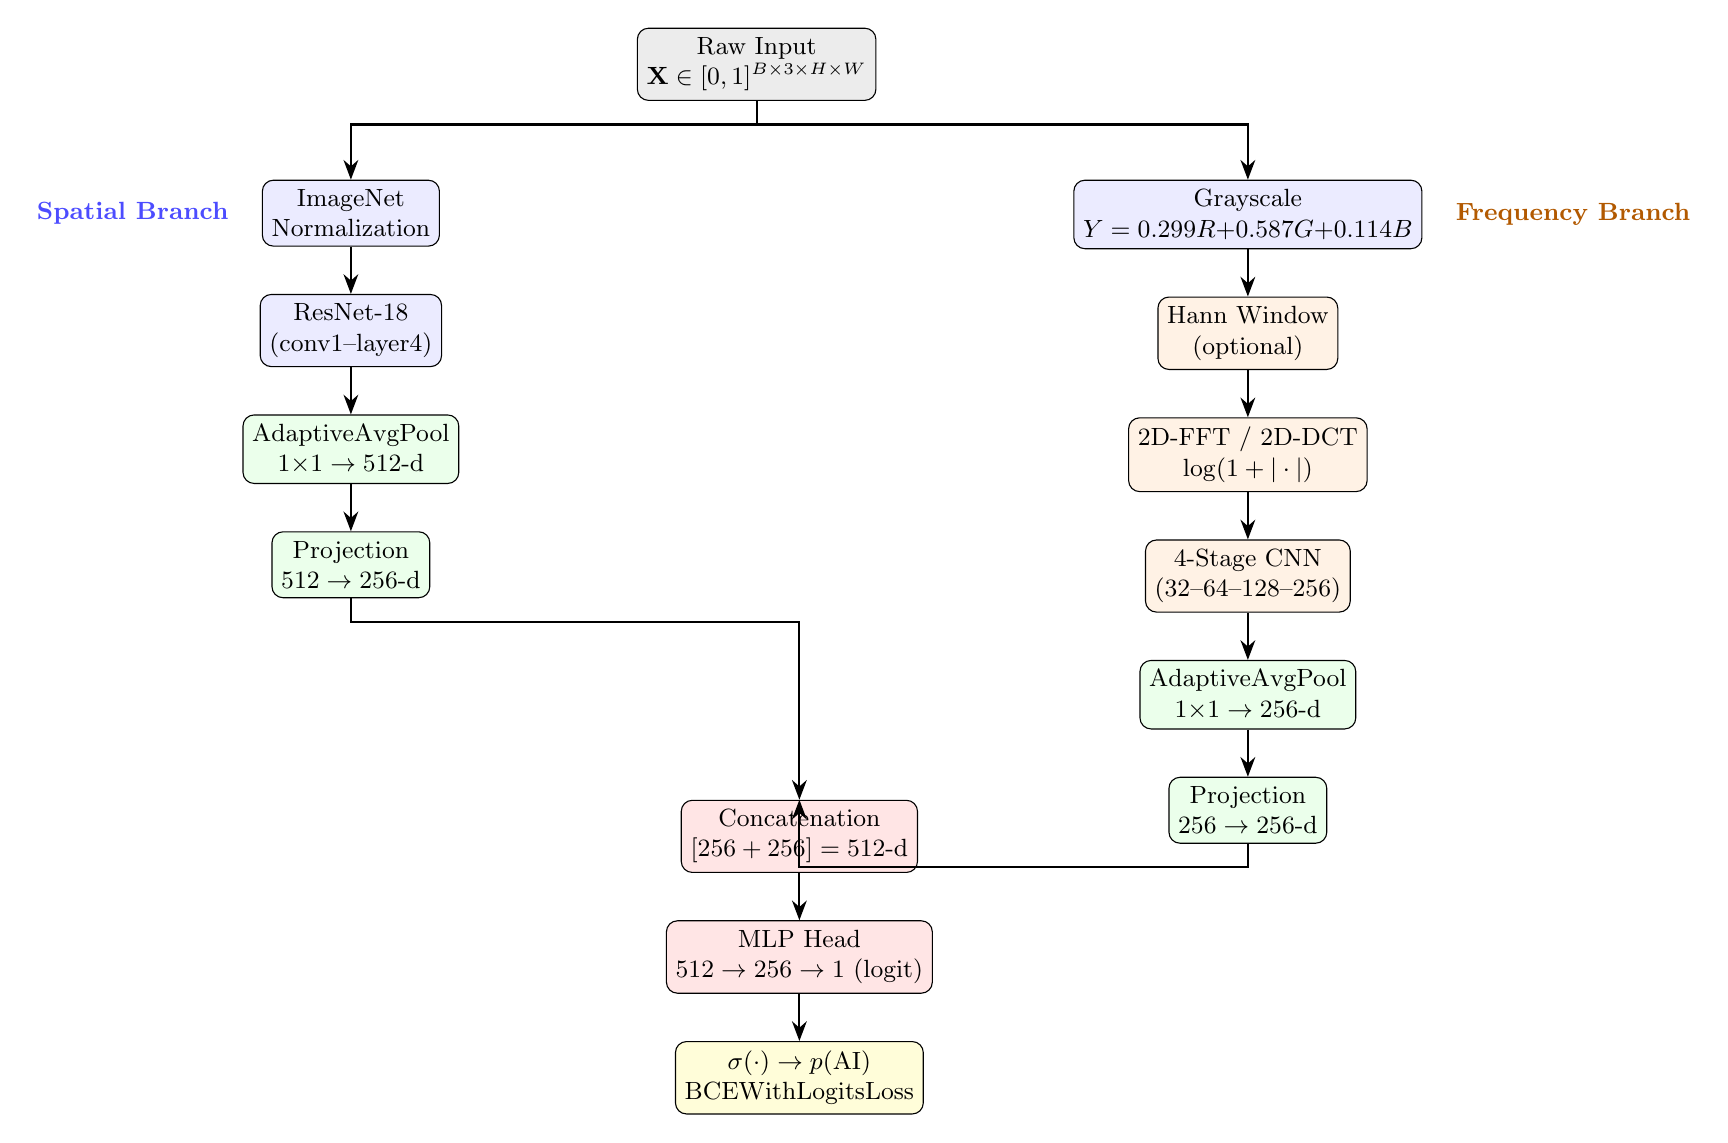
\begin{tikzpicture}[
    node distance=0.6cm and 0.8cm,
    block/.style={draw, rounded corners, fill=blue!8, minimum width=2.0cm, minimum height=0.7cm, font=\small, align=center},
    proc/.style={draw, rounded corners, fill=green!8, minimum width=1.8cm, minimum height=0.7cm, font=\small, align=center},
    spec/.style={draw, rounded corners, fill=orange!10, minimum width=1.8cm, minimum height=0.7cm, font=\small, align=center},
    arr/.style={-{Stealth[length=2.5mm]}, thick},
]

% Input
\node[block, fill=gray!15, minimum width=3cm] (input) {Raw Input\\$\mathbf{X} \in [0,1]^{B \times 3 \times H \times W}$};

% Branches split
\node[block, below left=1.0cm and 2.5cm of input] (spatial_norm) {ImageNet\\Normalization};
\node[block, below right=1.0cm and 2.5cm of input] (gray) {Grayscale\\$Y=0.299R{+}0.587G{+}0.114B$};

% Spatial path
\node[block, below=0.6cm of spatial_norm] (resnet) {ResNet-18\\(conv1--layer4)};
\node[proc, below=0.6cm of resnet] (gap1) {AdaptiveAvgPool\\$1{\times}1 \to 512$-d};
\node[proc, below=0.6cm of gap1] (sproj) {Projection\\$512 \to 256$-d};

% Frequency path
\node[spec, below=0.6cm of gray] (hann) {Hann Window\\(optional)};
\node[spec, below=0.6cm of hann] (transform) {2D-FFT / 2D-DCT\\$\log(1+|\cdot|)$};
\node[spec, below=0.6cm of transform] (fcnn) {4-Stage CNN\\(32--64--128--256)};
\node[proc, below=0.6cm of fcnn] (gap2) {AdaptiveAvgPool\\$1{\times}1 \to 256$-d};
\node[proc, below=0.6cm of gap2] (fproj) {Projection\\$256 \to 256$-d};

% Fusion
\node[block, fill=red!10, minimum width=3cm, below=1.0cm of $(sproj.south)!0.5!(fproj.south)$] (concat) {Concatenation\\$[256 + 256] = 512$-d};
\node[block, fill=red!10, below=0.6cm of concat] (head) {MLP Head\\$512 \to 256 \to 1$ (logit)};
\node[block, fill=yellow!15, below=0.6cm of head] (output) {$\sigma(\cdot) \to p(\text{AI})$\\BCEWithLogitsLoss};

% Arrows
\draw[arr] (input.south) -- ++(0,-0.3) -| (spatial_norm.north);
\draw[arr] (input.south) -- ++(0,-0.3) -| (gray.north);
\draw[arr] (spatial_norm) -- (resnet);
\draw[arr] (resnet) -- (gap1);
\draw[arr] (gap1) -- (sproj);
\draw[arr] (gray) -- (hann);
\draw[arr] (hann) -- (transform);
\draw[arr] (transform) -- (fcnn);
\draw[arr] (fcnn) -- (gap2);
\draw[arr] (gap2) -- (fproj);
\draw[arr] (sproj.south) -- ++(0,-0.3) -| (concat.north);
\draw[arr] (fproj.south) -- ++(0,-0.3) -| (concat.north);
\draw[arr] (concat) -- (head);
\draw[arr] (head) -- (output);

% Labels
\node[left=0.3cm of spatial_norm, font=\small\bfseries, text=blue!70] {Spatial Branch};
\node[right=0.3cm of gray, font=\small\bfseries, text=orange!70!black] {Frequency Branch};

\end{tikzpicture}
\caption{Architecture of the proposed dual-branch spatial-frequency fusion detector. The spatial branch applies ImageNet normalization and extracts features through a pre-trained ResNet-18, while the frequency branch computes a Hann-windowed 2D-FFT or separable 2D-DCT spectrum and processes it with a lightweight CNN. Both branches use adaptive global average pooling for resolution-agnostic operation. Features are projected to matched dimensionality and concatenated before the classification head.}
\label{fig:architecture}
\end{figure*}

\subsection{Data Ingestion and Deduplication}

Each dataset is downloaded and inspected using a depth-limited directory walk. Folder-to-label mappings are verified programmatically against the inspection output; ambiguous folder names trigger an explicit error rather than silent assignment. For every image file, we compute a SHA-256 hash on the raw bytes \emph{before} any crop or format conversion. Exact duplicates within the training partition are removed, and any validation or test sample whose hash collides with a training hash is purged. After deduplication, we assert zero hash overlap between train, validation, and test partitions. For datasets shipping predefined train/test splits (e.g., CIFAKE), we preserve those boundaries and carve a 15\% stratified validation set from the training partition; for datasets without splits, we apply seeded stratified 70/15/15 partitioning.

\subsection{Lossless Center-Crop Preprocessing}

A design principle of this work is that \emph{no interpolation} is applied at any stage. Resizing introduces resampling artifacts---downscaling aliases and low-passes the spectrum, while upscaling adds near-zero spectral energy---that contaminate the frequency features the detector targets. Instead, we apply a deterministic center-crop at the native pixel grid:
\begin{equation}
\label{eq:crop}
\mathbf{X}_{\text{crop}} = \mathbf{X}\!\left[\,\left\lfloor\tfrac{H-C}{2}\right\rfloor : \left\lfloor\tfrac{H-C}{2}\right\rfloor + C,\;\left\lfloor\tfrac{W-C}{2}\right\rfloor : \left\lfloor\tfrac{W-C}{2}\right\rfloor + C\,\right]
\end{equation}
where $C$ is the crop dimension, configured per dataset (224 for GRAVEX, FACES, CASHBOWMAN; 32 for CIFAKE). Images smaller than $C$ are skipped. Cropped patches are saved as lossless PNG to avoid JPEG re-encoding artifacts.

We define two evaluation protocols. \textbf{Protocol~N} (native) uses the per-dataset crop size for in-domain evaluation. \textbf{Protocol~C} (common) applies a secondary lossless center-crop to $32{\times}32$---the largest dimension every dataset supports---enabling spectral comparisons at identical resolution. Protocol~C is the primary metric for cross-dataset experiments because frequency statistics at different $N$ are not directly comparable.

\subsection{Spatial Branch}

The spatial branch receives a raw $[0, 1]$ RGB tensor and applies ImageNet normalization \emph{internally} as a registered buffer operation:
\begin{equation}
\label{eq:imagenet_norm}
\hat{\mathbf{X}}_c = \frac{\mathbf{X}_c - \mu_c}{\sigma_c}, \quad c \in \{R, G, B\}
\end{equation}
with $\boldsymbol{\mu} = [0.485, 0.456, 0.406]$ and $\boldsymbol{\sigma} = [0.229, 0.224, 0.225]$. Features are extracted through a pre-trained ResNet-18~\cite{he2016resnet} backbone (conv1 through layer4) followed by adaptive global average pooling, yielding a 512-dimensional embedding. The classification head is removed, and all convolutional weights are fine-tuned.

\subsection{Frequency Branch}

The frequency branch converts the raw $[0, 1]$ RGB input to luminance-weighted grayscale:
\begin{equation}
\label{eq:grayscale}
Y = 0.299\,R + 0.587\,G + 0.114\,B
\end{equation}

An optional 2D Hann window attenuates boundary discontinuities before spectral transformation:
\begin{equation}
\label{eq:hann}
w(n, m) = \sin^2\!\left(\frac{\pi n}{N}\right)\,\sin^2\!\left(\frac{\pi m}{M}\right)
\end{equation}
applied element-wise to the grayscale image: $\tilde{Y} = Y \odot w$.

The windowed image is then transformed by one of two spectral representations:

\textbf{2D-FFT.} The orthonormal 2D fast Fourier transform is applied via \texttt{torch.fft.rfft2} with subsequent \texttt{fftshift} along the vertical axis to center the zero-frequency component.

\textbf{Separable 2D-DCT-II.} We construct an orthonormal DCT-II matrix $\mathbf{D} \in \mathbb{R}^{N \times N}$:
\begin{equation}
\label{eq:dct}
D_{k,n} = s_k \cos\!\left(\frac{\pi(2n+1)k}{2N}\right), \quad s_k = \begin{cases} \sqrt{1/N} & k = 0 \\ \sqrt{2/N} & k \geq 1 \end{cases}
\end{equation}
and compute the 2D transform as the separable product $\mathbf{C} = \mathbf{D}\,\mathbf{X}\,\mathbf{D}^\mathsf{T}$. The matrix $\mathbf{D}$ is registered as a non-trainable buffer, built once per unique~$N$ and cached. This formulation avoids the $O(N^4)$ memory cost of an explicit Kronecker product and is validated against \texttt{scipy.fft.dctn(norm="ortho")} with a maximum absolute error below $5 \times 10^{-7}$.

Both transforms are followed by log-scale dynamic range compression and per-image min-max normalization:
\begin{equation}
\label{eq:logspec}
\mathbf{S} = \frac{\log(1 + |\mathbf{F}|) - \min}{\max - \min}
\end{equation}
where $\mathbf{F}$ denotes the FFT or DCT coefficient matrix and the normalization operates per sample.

The resulting single-channel spectral map is processed by a 4-stage CNN: four sequential blocks of $3{\times}3$ convolution, batch normalization, and ReLU, with $2{\times}2$ max-pooling between blocks. Channel widths progress as $1 \to 32 \to 64 \to 128 \to 256$. Adaptive global average pooling reduces the final feature map to a 256-dimensional vector.

\subsection{Fusion and Classification}

When projection is enabled (default), each branch embedding is mapped through a \mbox{Linear $\to$ BatchNorm $\to$ ReLU} layer to a common 256-dimensional space. The projected embeddings are concatenated into a 512-dimensional vector and passed to the classification head:
\begin{equation}
\label{eq:fusion}
\hat{y} = \mathbf{W}_2\,\phi\!\left(\text{BN}\!\left(\mathbf{W}_1\,[\mathbf{z}_s \,\|\, \mathbf{z}_f] + \mathbf{b}_1\right)\right) + b_2
\end{equation}
where $\phi$ is ReLU, $\|$ denotes concatenation, $\mathbf{W}_1 \in \mathbb{R}^{256 \times 512}$, $\mathbf{W}_2 \in \mathbb{R}^{1 \times 256}$, and dropout (rate 0.4) is applied before the final linear layer. The raw logit $\hat{y}$ is supervised with binary cross-entropy with logits loss. During ablation, the ``spatial\_only'' mode drops $\mathbf{z}_f$, ``freq\_only'' drops $\mathbf{z}_s$, and the head input dimension adjusts accordingly.

% ── Algorithm ─────────────────────────────────────────────────────────────────
\begin{algorithm}[t]
\caption{Training and Evaluation Protocol}
\label{alg:training}
\begin{algorithmic}[1]
\renewcommand{\algorithmicrequire}{\textbf{Input:}}
\renewcommand{\algorithmicensure}{\textbf{Output:}}
\REQUIRE Training set $\mathcal{D}_{\text{train}}$, validation set $\mathcal{D}_{\text{val}}$, test set $\mathcal{D}_{\text{test}}$, seeds $\mathcal{S} = \{42, 123, 2025\}$
\ENSURE Per-seed test metrics, aggregated mean $\pm$ std
\FOR{$s \in \mathcal{S}$}
    \STATE Set global seed $s$ (Python, NumPy, PyTorch, CUDA)
    \STATE Initialize FusedDetector $f_\theta$ with pre-trained ResNet-18
    \STATE Initialize AdamW optimizer ($\eta = 10^{-4}$, $\lambda = 10^{-2}$)
    \STATE Initialize CosineAnnealingLR scheduler ($T_{\max} = 20$, $\eta_{\min} = 10^{-6}$)
    \FOR{epoch $= 1$ \textbf{to} $E_{\max} = 20$}
        \STATE Train with AMP, gradient clipping $\|\nabla\| \leq 1.0$
        \STATE Evaluate on $\mathcal{D}_{\text{val}}$; record ROC-AUC
        \IF{val AUC improves}
            \STATE Save checkpoint; reset patience counter
        \ELSE
            \STATE Increment patience; \textbf{break} if patience $\geq 5$
        \ENDIF
        \STATE Step scheduler
    \ENDFOR
    \STATE Load best checkpoint
    \STATE Compute Youden's $J$ threshold on $\mathcal{D}_{\text{val}}$:
    \STATE \quad $\tau^* = \arg\max_\tau [\text{TPR}(\tau) - \text{FPR}(\tau)]$
    \STATE Evaluate on $\mathcal{D}_{\text{test}}$ with frozen $\tau^*$
\ENDFOR
\STATE Aggregate metrics: mean $\pm$ std over $|\mathcal{S}|$ seeds
\end{algorithmic}
\end{algorithm}


% ══════════════════════════════════════════════════════════════════════════════
%  IV. EXPERIMENTAL SETUP
% ══════════════════════════════════════════════════════════════════════════════

\section{Experimental Setup}
\label{sec:setup}

\subsection{Datasets}

We evaluate on four publicly available Kaggle datasets spanning distinct generative paradigms and resolutions:

\begin{enumerate}[leftmargin=*,nosep]
\item \textbf{GRAVEX-200K}~(``200k Real vs AI Visuals''): mixed photorealistic and diffusion-synthesized images at resolutions up to $1024{\times}1024$. Crop: $224{\times}224$. Used as the primary training source.
\item \textbf{140K Real and Fake Faces}~(``140k-real-and-fake-faces''): StyleGAN-generated faces paired with FFHQ real photographs at $1024{\times}1024$. Crop: $224{\times}224$.
\item \textbf{CASHBOWMAN}~(``ai-generated-images-vs-real-images''): mixed Midjourney and Stable Diffusion outputs at heterogeneous resolutions. Crop: $224{\times}224$.
\item \textbf{CIFAKE}~(``cifake-real-and-ai-generated-synthetic-images''): autoencoder-synthesized CIFAR-10 analogues at $32{\times}32$ native resolution. Crop: $32{\times}32$.
\end{enumerate}

After SHA-256 deduplication and class-balanced subsampling (up to 20{,}000 images per class), the aggregate corpus consists of 120{,}652 training, 64{,}900 validation, and 69{,}712 test images across all four datasets. Zero hash overlap is verified programmatically before any training commences.

\subsection{Implementation Details}

Training is conducted on a single NVIDIA Tesla T4 GPU (16~GB VRAM) in Google Colab. Table~\ref{tab:hyperparams} lists the full hyperparameter configuration. All experiments use mixed-precision training via PyTorch AMP with gradient clipping at $\|\nabla\| \leq 1.0$. The optimizer is AdamW~\cite{loshchilov2019adamw} with decoupled weight decay of $10^{-2}$ and a cosine annealing schedule from $10^{-4}$ to $10^{-6}$ over 20 epochs. Early stopping halts training if validation ROC-AUC does not improve for 5 consecutive epochs.

\begin{table}[t]
\caption{Hyperparameter Configuration}
\label{tab:hyperparams}
\centering
\begin{tabular}{ll}
\toprule
\textbf{Parameter} & \textbf{Value} \\
\midrule
Backbone & ResNet-18 (ImageNet pre-trained) \\
Batch size & 64 \\
Optimizer & AdamW ($\eta{=}10^{-4}$, $\lambda{=}10^{-2}$) \\
Scheduler & CosineAnnealingLR ($T_{\max}{=}20$) \\
Max epochs & 20 \\
Early stopping patience & 5 (on val ROC-AUC) \\
Gradient clipping & $\|\nabla\|_2 \leq 1.0$ \\
Mixed precision & FP16 (PyTorch AMP) \\
Projection dimension & 256 \\
Freq.\ CNN channels & 32--64--128--256 \\
Dropout (fusion head) & 0.4 \\
Hann window & Enabled (default) \\
Seeds & $\{42, 123, 2025\}$ \\
Protocol~C crop & $32 \times 32$ \\
Loss function & BCEWithLogitsLoss \\
\bottomrule
\end{tabular}
\end{table}

\subsection{Evaluation Metrics}

We report five metrics. \textbf{ROC-AUC} and \textbf{PR-AUC} are threshold-free and serve as primary ranking criteria. \textbf{Accuracy}, \textbf{F1-score}, and the classification report (precision, recall) are reported at two thresholds: the default 0.5 and the validation-calibrated Youden's~$J$ statistic~\cite{youden1950index}:
\begin{equation}
\label{eq:youden}
\tau^* = \arg\max_\tau \left[\text{TPR}(\tau) - \text{FPR}(\tau)\right]
\end{equation}
computed exclusively on the validation set. The same $\tau^*$ is applied unchanged to the test set and all cross-dataset targets. Per-image inference latency is measured after 10 GPU warm-up passes, averaged over 50 forward passes at batch sizes 1 and 64.

\subsection{Experimental Design}

We conduct six experiment groups:
\begin{itemize}[leftmargin=*,nosep]
\item \textbf{E1--E3}: Architecture ablation on GRAVEX (spatial-only, frequency-only, fused with FFT and fused with DCT), each with three seeds.
\item \textbf{E4}: Hann window ablation (fused FFT with and without windowing).
\item \textbf{E5}: Computational profiling (parameter counts, inference latency).
\item \textbf{E6}: Zero-shot cross-dataset transfer from GRAVEX to FACES, CASHBOWMAN, and CIFAKE under both Protocol~C and Protocol~N.
\end{itemize}


% ══════════════════════════════════════════════════════════════════════════════
%  V. RESULTS AND DISCUSSION
% ══════════════════════════════════════════════════════════════════════════════

\section{Results and Discussion}
\label{sec:results}

\subsection{In-Domain Architecture Ablation (E1--E4)}

Table~\ref{tab:ablation} presents the in-domain results on the GRAVEX test split. The fused DCT variant achieves the highest ROC-AUC of 0.9268, with the spatial-only baseline at 0.9255 and the frequency-only branch at 0.7021. The fused FFT variant with Hann windowing reaches 0.9247, while the same configuration without windowing obtains 0.9245---a marginal difference suggesting that for FFT on center-cropped images, spectral leakage from boundary discontinuities is a secondary concern compared to the inherent spectral structure.

\begin{table}[t]
\caption{In-Domain Ablation on GRAVEX Test Set (mean $\pm$ std over seeds)}
\label{tab:ablation}
\centering
\resizebox{\columnwidth}{!}{%
\begin{tabular}{lcccc}
\toprule
\textbf{Variant} & \textbf{Seeds} & \textbf{Accuracy} & \textbf{ROC-AUC} & \textbf{F1} \\
\midrule
Spatial-only (ResNet-18)     & 3 & 0.8451 $\pm$ 0.0012 & 0.9255 $\pm$ 0.0011 & 0.8469 $\pm$ 0.0014 \\
Freq-only (FFT+Hann)         & 3 & 0.6486 $\pm$ 0.0025 & 0.7021 $\pm$ 0.0026 & 0.6510 $\pm$ 0.0091 \\
Fused FFT+Hann               & 4 & 0.8455 $\pm$ 0.0002 & 0.9247 $\pm$ 0.0002 & 0.8469 $\pm$ 0.0006 \\
Fused FFT (no Hann)           & 1 & 0.8439              & 0.9245              & 0.8412              \\
\textbf{Fused DCT+Hann}       & 1 & \textbf{0.8473}     & \textbf{0.9268}     & \textbf{0.8508}     \\
\bottomrule
\end{tabular}%
}
\end{table}

The frequency-only branch's ROC-AUC of 0.7021 indicates that spectral features alone, while informative, lack the discriminative granularity of spatial texture and edge statistics when operating on diverse photorealistic content. The fused architecture overcomes this limitation by allowing the classification head to weight complementary cues from both domains. The DCT variant's slight advantage over FFT (0.9268 vs.\ 0.9247) is consistent with Bilbis~\emph{et~al.}'s observation~\cite{bilbis2025dctvsfft} that DCT's block-aligned basis functions capture localized spectral energy distributions that are more stable under perturbation.

The standard deviations across seeds---below 0.003 for all metrics in the fused configurations---confirm the stability of the training procedure under the controlled seed protocol.

\subsection{Computational Efficiency (E5)}

Table~\ref{tab:efficiency} reports parameter counts and inference latencies. The fused model contains 11.96M trainable parameters, only 0.10M more than the spatial-only variant (11.86M), because the frequency branch's 4-stage CNN (0.10M parameters) is substantially lighter than the ResNet-18 backbone. At batch size~64, the fused model processes each image in 0.132--0.154~ms, corresponding to a throughput exceeding 6{,}400~images/second on a single T4 GPU---well within real-time operational requirements.

\begin{table}[t]
\caption{Computational Efficiency Comparison}
\label{tab:efficiency}
\centering
\resizebox{\columnwidth}{!}{%
\begin{tabular}{lccc}
\toprule
\textbf{Variant} & \textbf{Params (M)} & \textbf{Lat.\ BS=1 (ms)} & \textbf{Lat.\ BS=64 (ms/img)} \\
\midrule
Freq-only (FFT)        & 11.86 & 2.76  & 0.046 \\
Spatial-only            & 11.86 & 5.99  & 0.085 \\
Fused FFT (no Hann)     & 11.96 & 7.70  & 0.138 \\
Fused FFT+Hann          & 11.96 & 7.68  & 0.132 \\
Fused DCT+Hann          & 11.96 & 9.13  & 0.154 \\
\bottomrule
\end{tabular}%
}
\end{table}

The DCT variant incurs a higher single-image latency (9.13~ms vs.\ 7.68~ms for FFT) due to the explicit matrix multiplications in the separable $\mathbf{D}\mathbf{X}\mathbf{D}^\mathsf{T}$ computation, whereas FFT leverages highly optimized CUDA kernels. At batch size~64, this overhead amortizes to 0.022~ms/image, rendering the difference operationally negligible.

\subsection{Cross-Dataset Generalization (E6)}

Table~\ref{tab:cross} presents zero-shot transfer results under Protocol~C ($32{\times}32$ common crop). The model is trained exclusively on GRAVEX and evaluated on the remaining three datasets without fine-tuning; the Youden threshold calibrated on the GRAVEX validation set is applied unchanged to all targets.

\begin{table}[t]
\caption{Zero-Shot Cross-Dataset Transfer (Protocol~C, $32{\times}32$)}
\label{tab:cross}
\centering
\resizebox{\columnwidth}{!}{%
\begin{tabular}{llcccc}
\toprule
\textbf{Target} & \textbf{Setting} & \textbf{Samples} & \textbf{ROC-AUC} & \textbf{PR-AUC} & \textbf{Acc.\ (\%)} \\
\midrule
GRAVEX      & In-Domain   & 29{,}991 & 0.9421 & 0.9433 & 87.03 \\
FACES       & Zero-Shot   & 20{,}000 & \textbf{0.9656} & \textbf{0.9683} & \textbf{90.97} \\
CASHBOWMAN  & Zero-Shot   & 137      & 0.4603 & 0.5773 & 54.01 \\
CIFAKE      & Zero-Shot   & 19{,}622 & 0.5001 & 0.4944 & 49.44 \\
\bottomrule
\end{tabular}%
}
\end{table}

The FACES result (0.9656 ROC-AUC, 90.97\% accuracy) demonstrates that the fused model captures generative artifacts that transfer across generative paradigms. GRAVEX contains diffusion-synthesized general-purpose images, while FACES consists of StyleGAN-generated human faces paired with FFHQ photographs---two fundamentally different generation pipelines and semantic domains. The high transfer accuracy suggests that both spatial texture anomalies (blurred skin pores, inconsistent hair strands) and spectral fingerprints (upsampling grid patterns, truncated high-frequency energy) are shared across these architectures despite their mechanistic differences.

The near-chance performance on CASHBOWMAN (0.4603 AUC, 137 test samples) and CIFAKE (0.5001 AUC) demands careful analysis. CASHBOWMAN's extremely small test partition limits statistical power; with only 137 images, the confidence interval on AUC spans approximately $\pm 0.08$ at 95\% confidence. CIFAKE's $32{\times}32$ native resolution represents a qualitatively different domain: images at this scale encode scene-level structure rather than fine-grained texture, and the spectral resolution (only $32 \times 32 = 1{,}024$ frequency bins) provides far fewer discriminative coefficients than the $224 \times 224 = 50{,}176$ bins available in GRAVEX training images. Under Protocol~C, all images are cropped to $32{\times}32$, equalizing the spectral resolution; however, the spatial features learned on GRAVEX's rich $224{\times}224$ textures do not transfer to CIFAKE's low-resolution object silhouettes. This spectral resolution mismatch constitutes the primary failure mode of cross-domain transfer in our framework.

\subsection{Limitations and Threats to Validity}

Several factors bound the generalizability of these results. First, the training source is a single dataset (GRAVEX-200K); multi-source training across generative paradigms would likely improve cross-domain robustness. Second, center-cropping preserves native pixel statistics but discards peripheral context and reduces the effective field of view, particularly for small crops. Third, while SHA-256 deduplication eliminates exact duplicates, near-duplicate detection (e.g., via perceptual hashing) was disabled in these experiments; subtle image variations below the perceptual threshold could inflate apparent test performance. Fourth, all datasets are sourced from Kaggle and may not represent the full diversity of in-the-wild synthetic media, which undergo social media compression, resizing, and screenshot re-encoding. Fifth, the resolution shortcut---if real images are natively larger than fakes within a dataset, the same center crop covers a different fraction of the scene, and scale-dependent sharpness cues may persist despite controlled cropping.


% ══════════════════════════════════════════════════════════════════════════════
%  VI. CONCLUSION
% ══════════════════════════════════════════════════════════════════════════════

\section{Conclusion and Future Work}
\label{sec:conclusion}

We presented a dual-branch architecture that fuses pre-trained ResNet-18 spatial features with lightweight CNN-processed 2D-FFT or separable 2D-DCT spectral representations for binary AI-generated image detection. The pipeline enforces lossless center-cropping, SHA-256 deduplication, and validation-only threshold calibration to maintain evaluation integrity. On the GRAVEX-200K in-domain test set, the fused DCT variant attains 0.9268 ROC-AUC, and zero-shot transfer to StyleGAN-generated faces yields 0.9656 ROC-AUC with 90.97\% accuracy---achieved without target-domain fine-tuning or data augmentation beyond horizontal flipping and light colour jitter.

The systematic ablation confirms that frequency features alone (0.7021 AUC) are insufficient for general detection, but their fusion with spatial features produces stable, seed-robust classifiers whose DCT variant marginally outperforms the FFT counterpart. The cross-dataset evaluation under Protocol~C reveals that spectral resolution mismatch between source and target domains, rather than model capacity, is the dominant barrier to universal detection.

Three directions merit further investigation. First, multi-source training incorporating heterogeneous generators and resolutions during the training phase could mitigate the resolution-mismatch failure mode observed on CIFAKE. Second, integrating compression-aware augmentation (controlled JPEG and WebP degradation applied \emph{before} frequency extraction) would better simulate real-world distribution channels, as Bilbis~\emph{et~al.}~\cite{bilbis2025dctvsfft} demonstrated the differential robustness of DCT features under JPEG compression. Third, replacing the fixed ResNet-18 backbone with a resolution-adaptive spectral pre-training strategy, as explored by Karageorgiou~\emph{et~al.}~\cite{karageorgiou2025spai}, could unify in-domain accuracy with cross-resolution generalization within a single model.


% ══════════════════════════════════════════════════════════════════════════════
%  REFERENCES
% ══════════════════════════════════════════════════════════════════════════════

\bibliographystyle{IEEEtran}
\bibliography{references}

\end{document}
